\section{Costruzione del Reticolo della Conoscenza}
\label{Costruzione del Reticolo della Conoscenza}
Dal 26/07  al 28/07 ho iniziato la Costruzione del Reticolo della Conoscenza. Per realizzarlo ho utilizzato un'applicativo sviluppato durante un precedente stage dell'azienda, che fa largo uso della libreria d3.js; effettuando elaborazione di dati presentandoli in \textit{Cluster Based} o \textit{Force Based}, a discrezione delle esigenze dell'utente.

\subsection{Descrizione del sistema}
\label{Descrizione del sistema}
L'applicazione accetta in import file di estensione CSV. Ogni colonna di quest'ultimo viene interpretata dal sistema come un parametro da elaborare; per questo la prima riga del file deve essere o preceduta da una dichiarazione di variabili, tante quante sono le colonne da parametrizzare, oppure \`e questa prima riga che viene interpretata come una dichiarazione e conseguentemente non rappresentata all'interno del Reticolo.\\
Nel sistema possono venire settati i seguenti aspetti:
\begin{itemize}
\item La \textit{tipologie} di Reticolo:
\begin{itemize}
\item Cluster Based: raggruppa un insieme di oggetti in modo tale che gli tutti gli elementi contenuti nel medesimo cluster sono pi\`u simili l'uno all'altro rispetto a quelli contenuti in altri gruppi;
\item Force Based: in base alla forza di ogni nodo viene rappresentata come unica regione compatta le istanze appartenenti alla medesima classe in cui vengono visivamente identificati i percorsi di differenziazione. Nel layout le celle differenzianti sono poste in prossimit\`a della classe pi\`u fortemente correlata.
\end{itemize}
\item \textit{Normalizzazione} dei dati in input:
\begin{itemize}
\item No: non viene applicata alcuna tecnica di normalizzazione dei dati;
\item MinMax: i dati vengono ridimensionati su un intervallo specifico (min, max), tuttavia tale tecnica non \`e in grado di gestire i valori anomali;
\item Gaussian: o normale in cui i dati vengono normalizzati in una curva in cui i valori della stessa grandezza sono soggetti ad approssimazione;
\item Interquartile: si occupa di standardizzare i dati in modo da quantificare l'estensione del 50\% della distribuzione del carattere che si trovano attorno alla mediana;
\end{itemize}
\item Tipologia di \textit{distanza} applicabili ai punti:
\begin{itemize}
\item Euclidea: tiene conto della distanza tra i punti;
\item Camberra: tiene conto della distanza tra le coppie in uno spazio vettoriale;
\item Pearson: distanza di correlazione che misura il grado di correlazione tra due punti. Valuta la covarianza tra due variabili in rapporto al prodotto della deviazione standard. Non \`e vantaggiosa su dati semplici.
\end{itemize}
\item \textit{Metodo} di associazione dei punti:
\begin{itemize}
\item Single: "vicino al prossimo", la distanza fra i gruppi \`e posta al pari della pi\`u piccola delle distanze calcolabili a due a due tra tutti gli elementi del gruppo. Accentua tutte le somiglianze tra i gruppi a discapito  della loro differenziazione netta.
\item Complete: "vicino pi\`u lontano", viene considerata la maggiore tra le distanze calcolate a due a due tra gli elementi di due gruppi. Privilegia la differenziazione tra i gruppi a discapito dell'omogeneit\`a degli elementi in essi contenuti. In questo caso i punti vengono rappresentati come meno compatti e diluiti.
\item Average: viene considerata come distanza fra due gruppi la media fra tutte le distanze calcolate a due a due tra gli elementi dei due gruppi. I risultati ottenibili sono i pi\`u attendibili (essendo basato sulla media delle distanze), i gruppi risultano pi\`u omogenei e differenziati tra di loro.
\end{itemize}
\end{itemize}
\noindent
Un'ulteriore funzionalit\`a permette all'utente di decidere se si desidera procedere con una rappresentazione del Reticolo manuale o automatica progressiva dei dati.

\subsubsection{Configurazione}
\label{configurazione}
Analizzando l'applicativo in base al carattere dei dati in ingresso e alle aspettative sull'output del modello, ho riscontrato che la configurazione necessaria per la formazione del Reticolo della Conoscenza \`e vincolata alla dischiarazione delle seguenti propriet\`a:
\begin{itemize}
\item \textit{Redistance}: No;
\item  \textit{Normalize}: No;
\item \textit{Distance-Type}: Euclidea;
\item \textit{Method}: Single.
\end{itemize}
\noindent
\begin{figure}[H]
\centering
	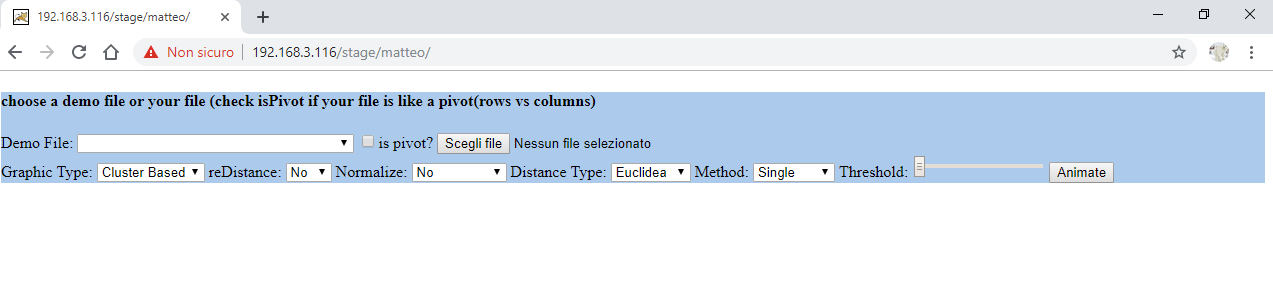
\includegraphics[width=1\linewidth]{./image/img-configurazione_reticolo.png}
	\caption{Configurazione usata nel sistema per generare il Reticolo della Conoscenza.}
	\label{Configurazione usata nel sistema per generare il Reticolo della Conoscenza.}
\end{figure}
\noindent

\section{Creazione dei file CSV}
\label{Creazione dei file CSV}
Come gi\`a accentato all'interno della sezione §\ref{Descrizione del sistema} prima di procedere alla creazione del Reticolo ho dovuto preparare i dati di previsione prima di poterli dare in pasto al sistema. Questo \`e stato reso pi\`u agevole grazie alla creazione, da parte mia, di un metodo che ha il compito, una volta messa in funzione la Rete neurale oggetto di studio (di prova o del database), di calcolare:
\begin{enumerate}
\item Le previsioni ottenibili da un vettore di previsione settato a 1 o -1 per ogni singolo elemento;
\item Sui dati del punto (1) un vettore delle differenze dove viene calcolato il delta in rapporto al vettore di standard \footnote{Vettore tutto a zero}.
\end{enumerate}
\noindent
Ho fatto in modo che il vettore delle differenze venga stampato su console del browser \footnote{unica alternativa facendo uso di solo codice javascript}, in modo che ne basti prelevare il contenuto e inserirlo su un file CSV. Ogni elemento per poter funzionare all'interno dell'applicativo deve essere separato da un ; e ogni riga di previsione deve essere preceduta dal codice della domande in modo da rendere pi\`u agevole l'interpretazione del Reticolo. \`E a discrezione dell'utente l'inserimento di un'ulteriore riga di dichiarazione dei parametri.

\section{Creazione del Reticolo della Conoscenza per sui dati di Prova}
\label{Creazione del Reticolo della Conoscenza per sui dati di Prova}
\noindent
\begin{figure}[H]
\centering
	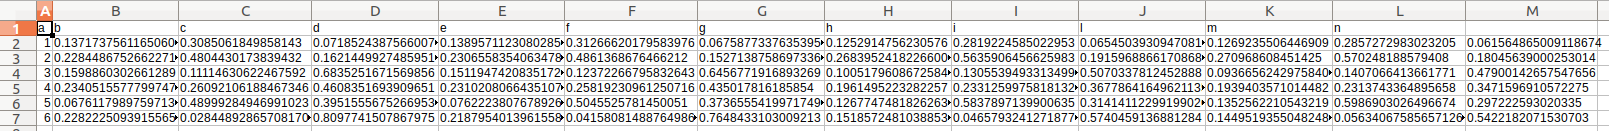
\includegraphics[width=1\linewidth]{./image/fileCSV_rete-prova.png}
	\caption{file CSV generato per la creazione del Reticolo della Conoscenza sui dati di prova.}
	\label{file CSV generato per la creazione del Reticolo della Conoscenza sui dati di prova.}
\end{figure}
\noindent
\textit{Di seguito sono riportate le sequenze di creazione del Reticolo della Conoscenza per i dati di prova.}
\noindent
\begin{figure}[H]
\centering
	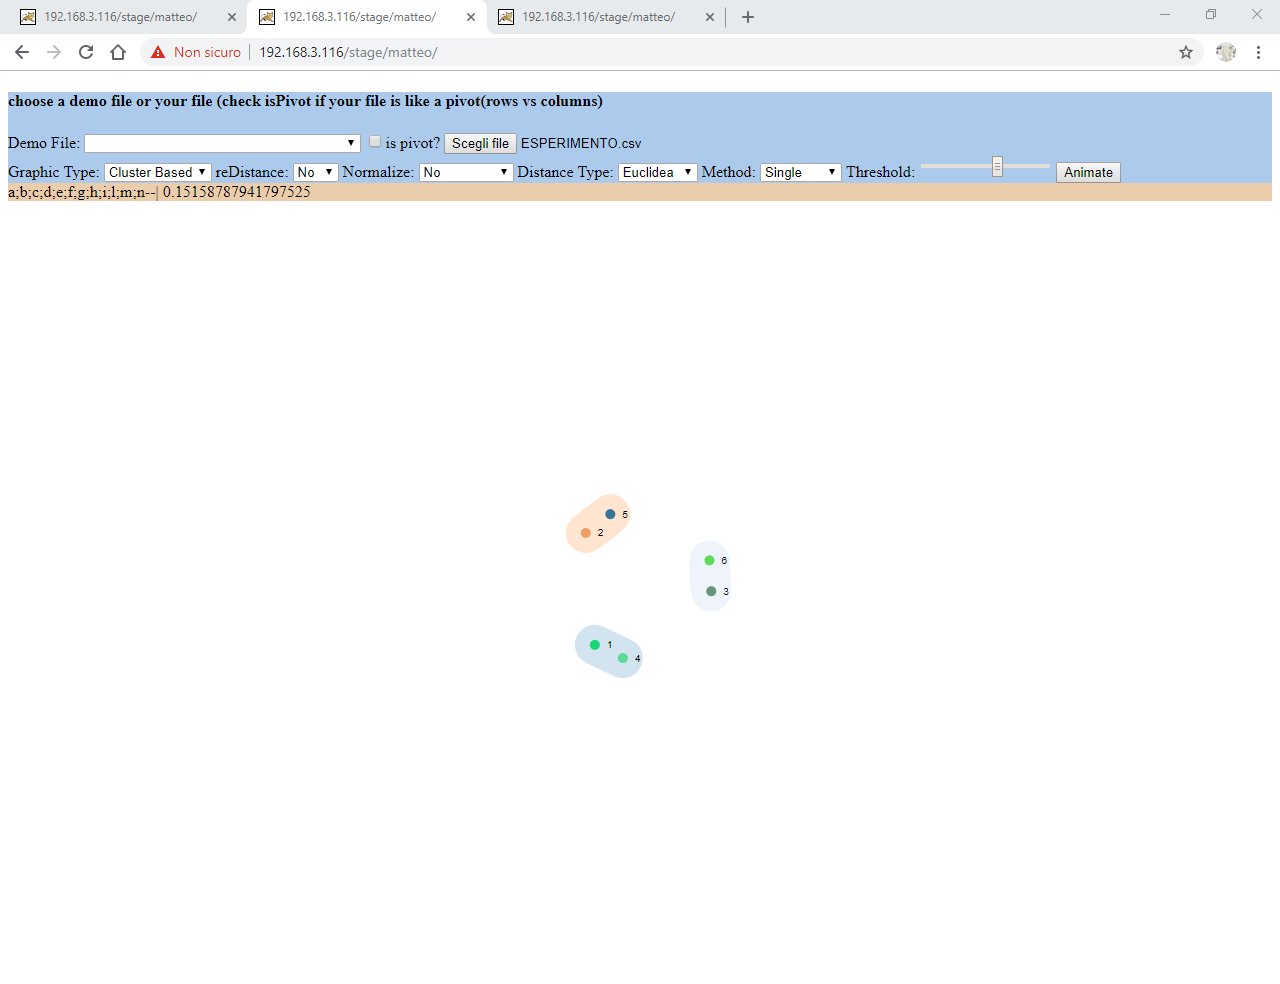
\includegraphics[width=1\linewidth]{./image/reticoloCorretto1.png}
	\caption{Reticolo della Conoscenza con rappresentazione di tipo Cluster Based - 1.}
	\label{Reticolo della Conoscenza con rappresentazione di tipo Cluster Based - 1.}
\end{figure}
\noindent
\begin{figure}[H]
\centering
	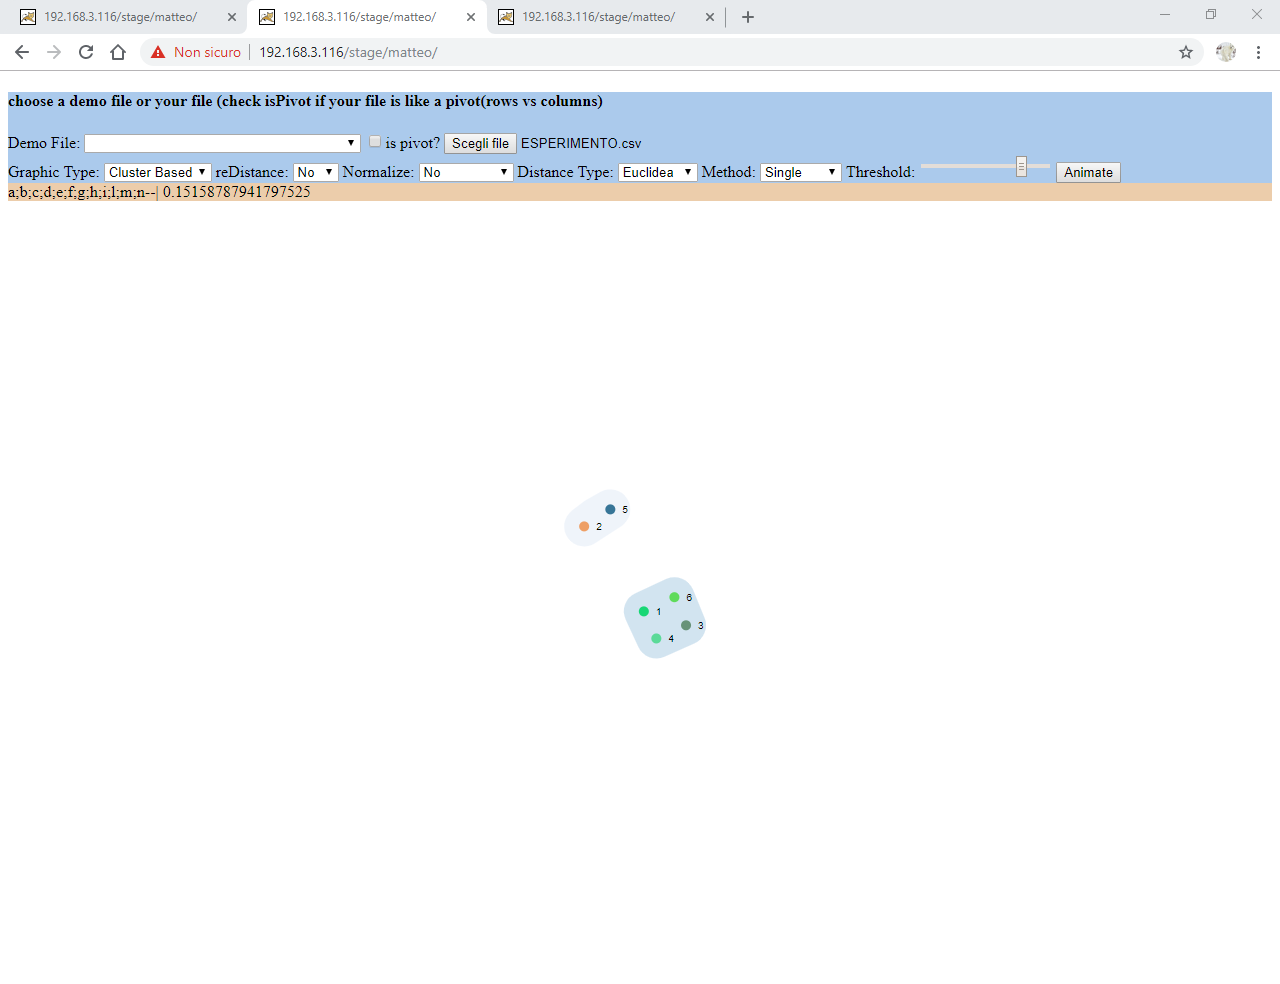
\includegraphics[width=1\linewidth]{./image/reticoloCorretto2.png}
	\caption{Reticolo della Conoscenza con rappresentazione di tipo Cluster Based - 2.}
	\label{Reticolo della Conoscenza con rappresentazione di tipo Cluster Based - 2.}
\end{figure}
\noindent
\begin{figure}[H]
\centering
	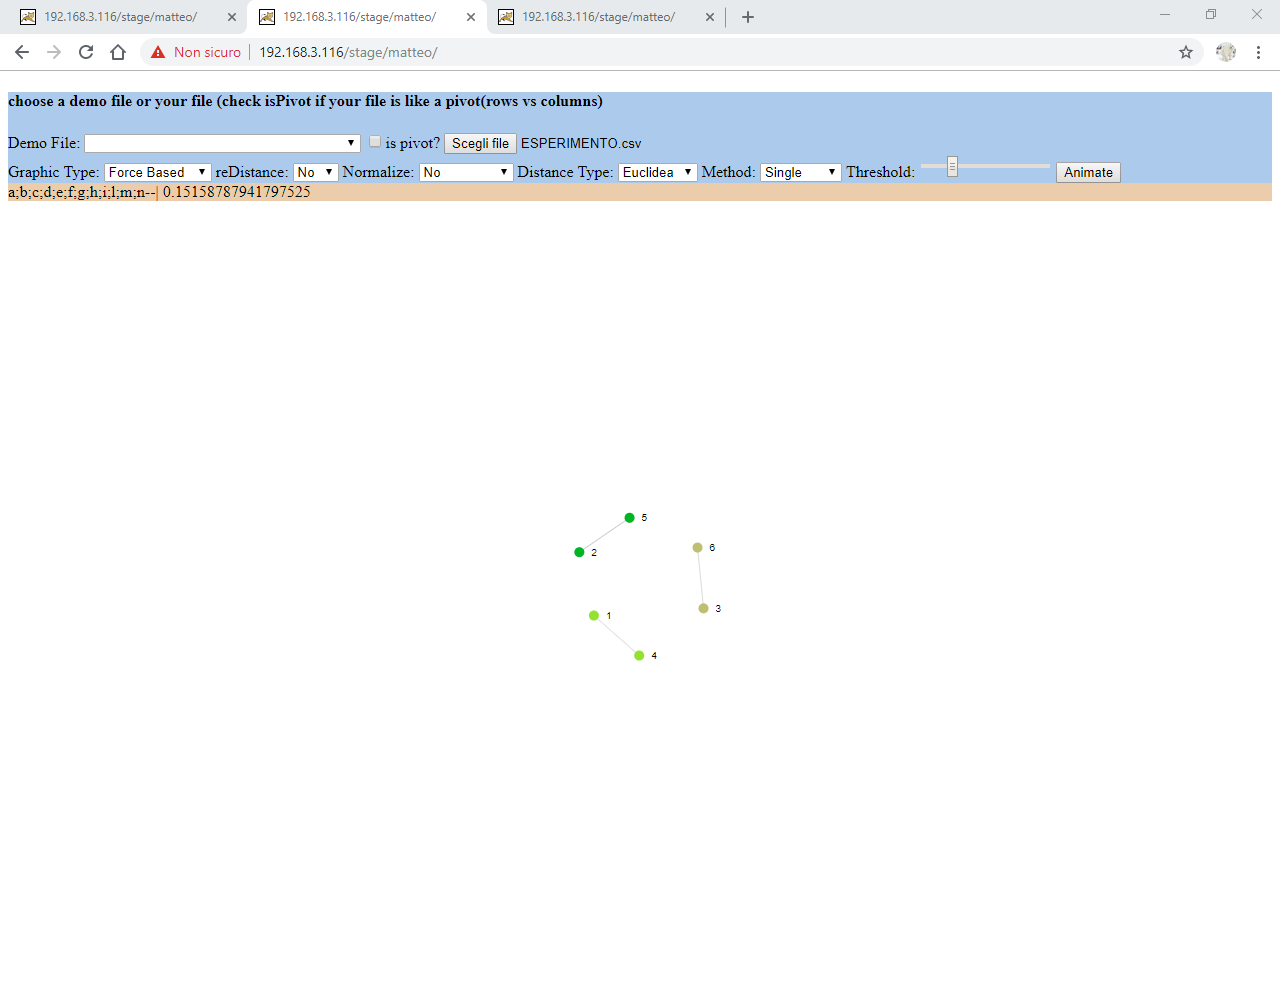
\includegraphics[width=1\linewidth]{./image/reticoloCorretto3.png}
	\caption{Reticolo della Conoscenza con rappresentazione di tipo Forced Based - 1.}
	\label{Reticolo della Conoscenza con rappresentazione di tipo Forced Based - 1.}
\end{figure}
\noindent
\begin{figure}[H]
\centering
	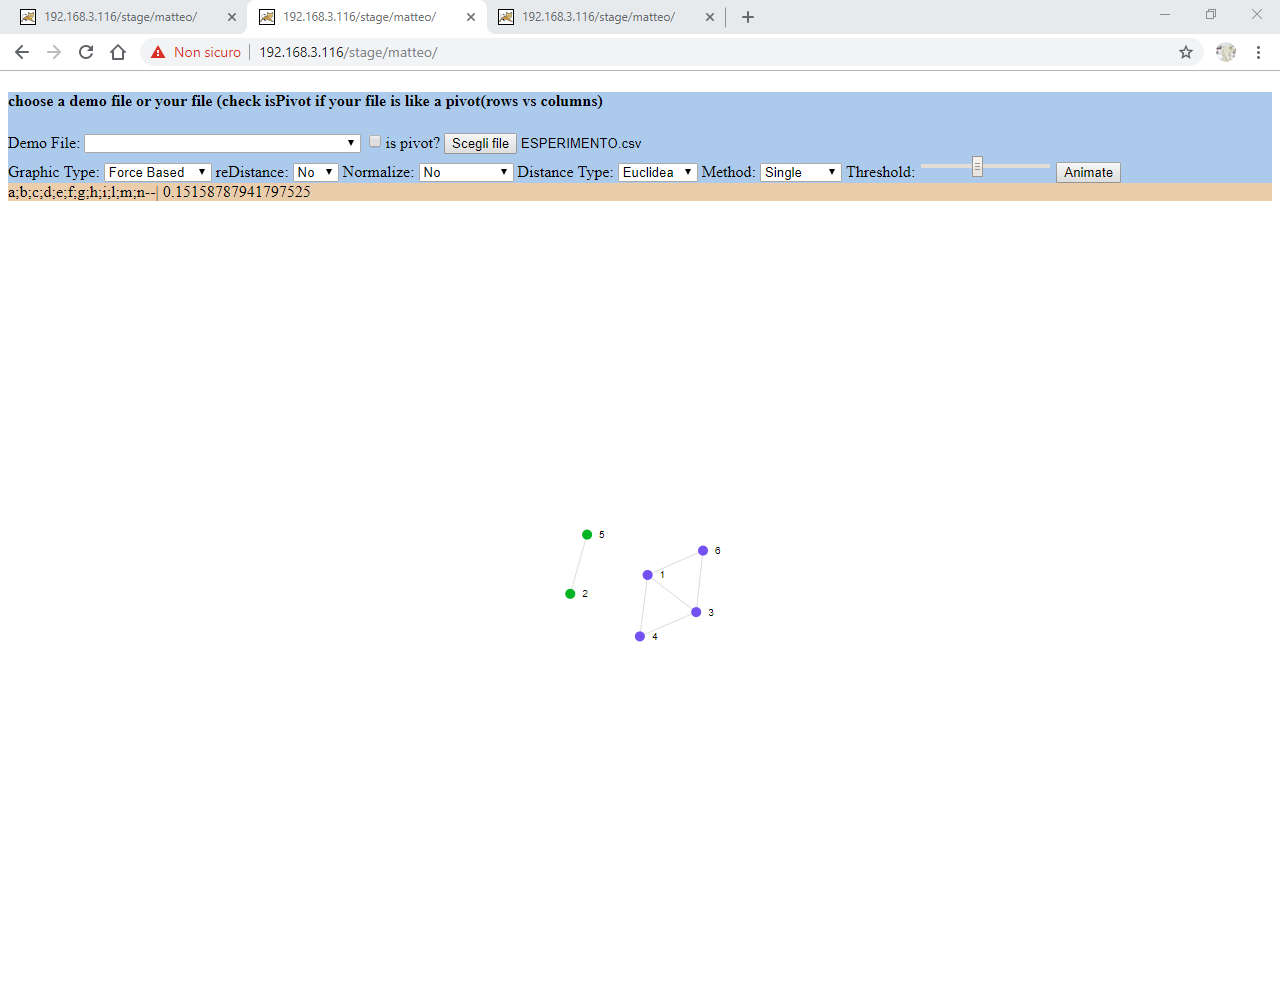
\includegraphics[width=1\linewidth]{./image/reticoloCorretto4.png}
	\caption{Reticolo della Conoscenza con rappresentazione di tipo Forced Based - 2.}
	\label{Reticolo della Conoscenza con rappresentazione di tipo Forced Based - 2.}
\end{figure}
\noindent
\begin{figure}[H]
\centering
	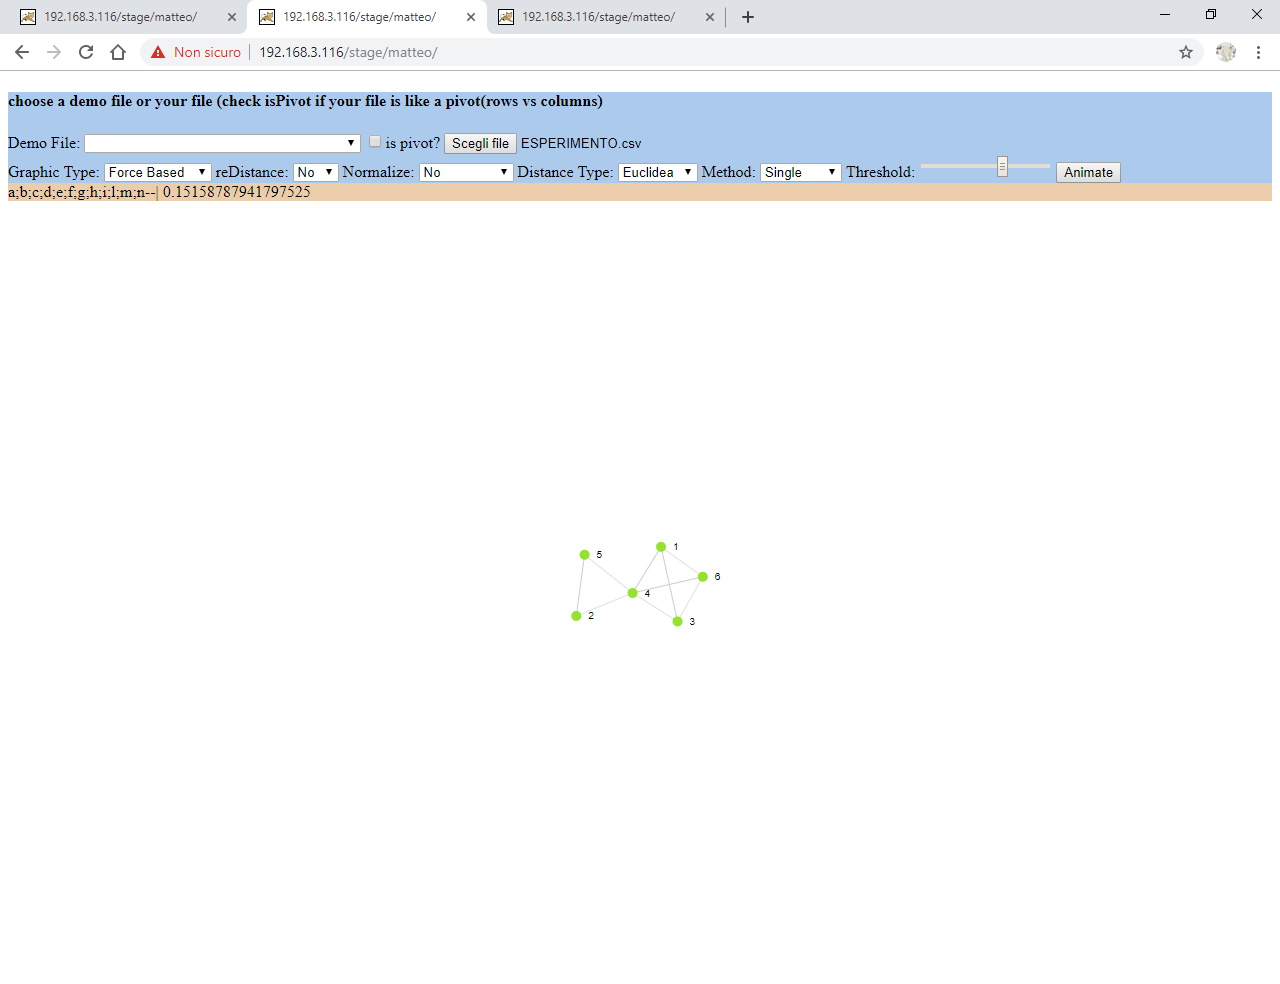
\includegraphics[width=1\linewidth]{./image/reticoloCorretto5.png}
	\caption{Reticolo della Conoscenza con rappresentazione di tipo Forced Based - 3.}
	\label{Reticolo della Conoscenza con rappresentazione di tipo Forced Based - 3.}
\end{figure}
\noindent
\textit{Appare evidente come il Reticolo generato rispetta quando definito dalla figura \ref{Grafo rappresentante le relazioni esistenti tra il set di domande di prova.}.\\
Tuttavia effettuando delle ulteriori prove con file dati differenti; ma provenienti dalla medesima Rete neurale ho riscontrato situazioni contrastanti. L'errore che si riscontra nei casi non corretti riguarda le coppie di domande 1, 4 e 3, 6. Un esempio del fenomeno \`e illustrato di seguito.}
\begin{figure}[H]
\centering
	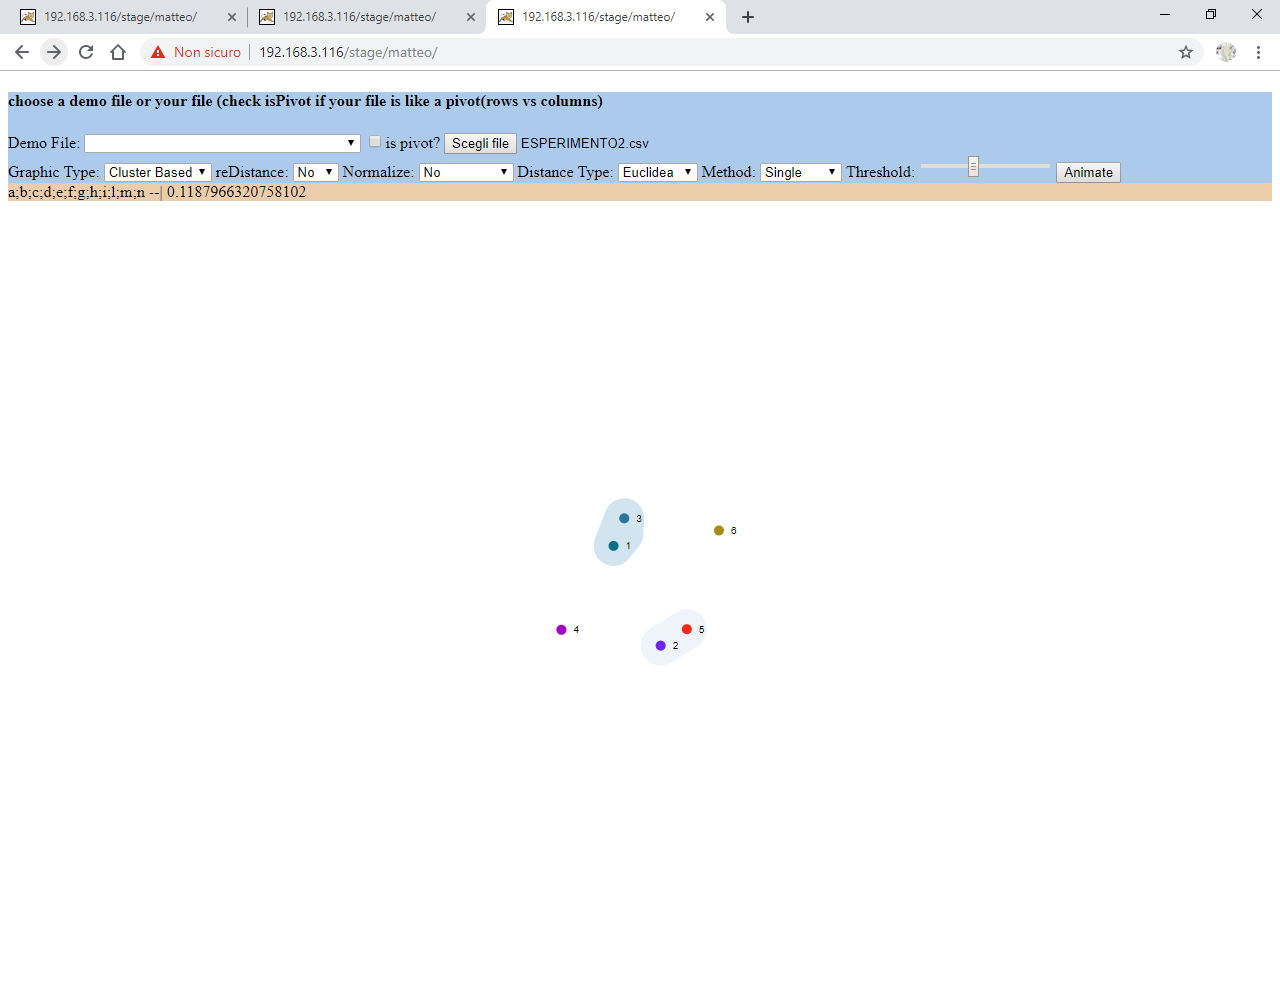
\includegraphics[width=1\linewidth]{./image/reticoloNonCorretto1.png}
	\caption{Reticolo della Conoscenza con rappresentazione di tipo Forced Based - 3.}
	\label{Reticolo della Conoscenza con rappresentazione di tipo Forced Based - 3.}
\end{figure}
\noindent\\
\begin{figure}[H]
\centering
	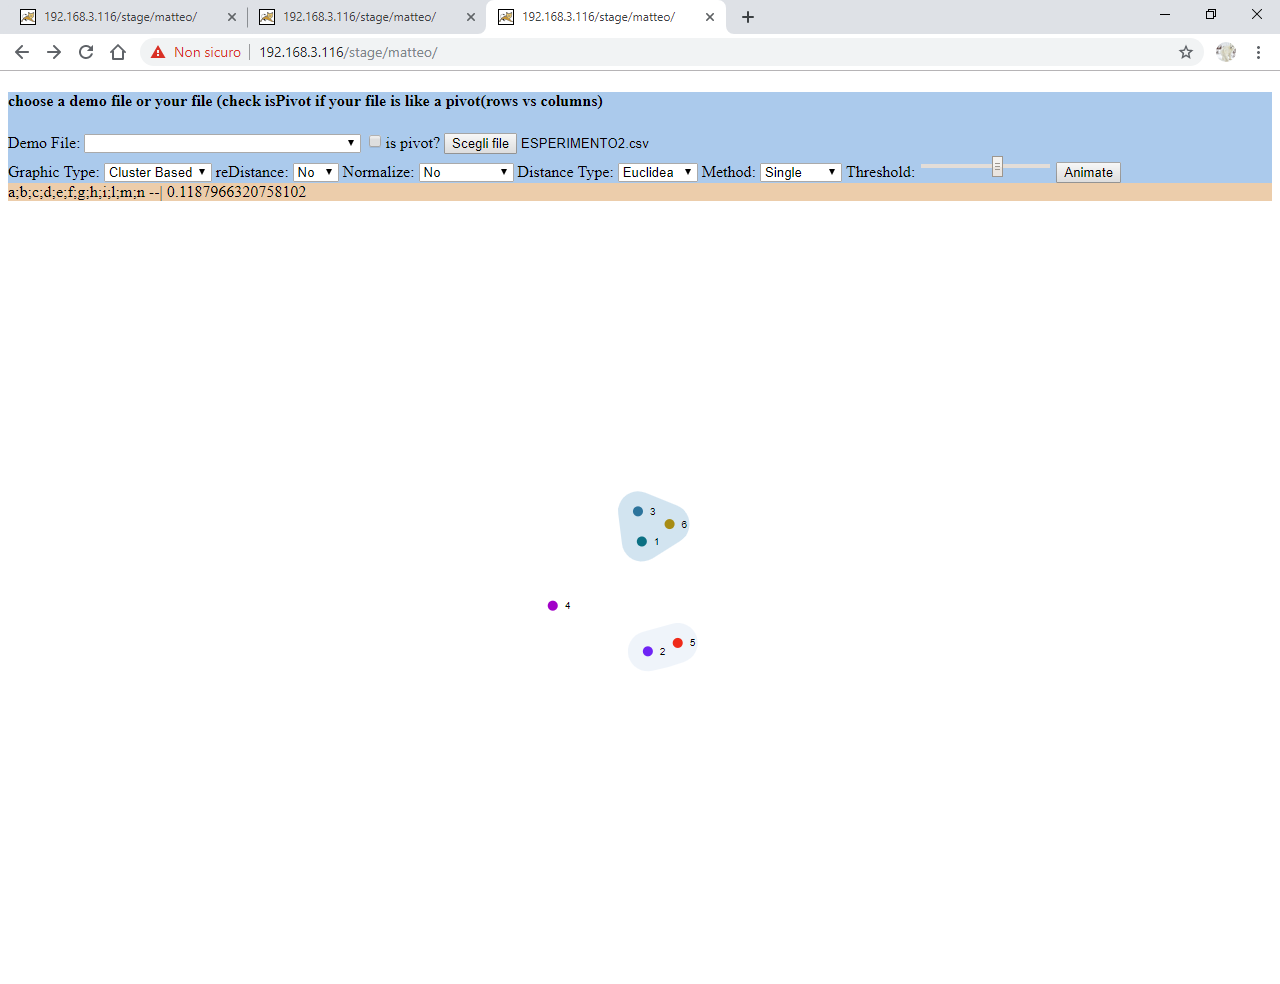
\includegraphics[width=1\linewidth]{./image/reticoloNonCorretto2.png}
	\caption{Reticolo della Conoscenza con rappresentazione di tipo Cluster Based - 1.}
	\label{Reticolo della Conoscenza con rappresentazione di tipo Cluster Based - 1.}
\end{figure}
\noindent\\
\begin{figure}[H]
\centering
	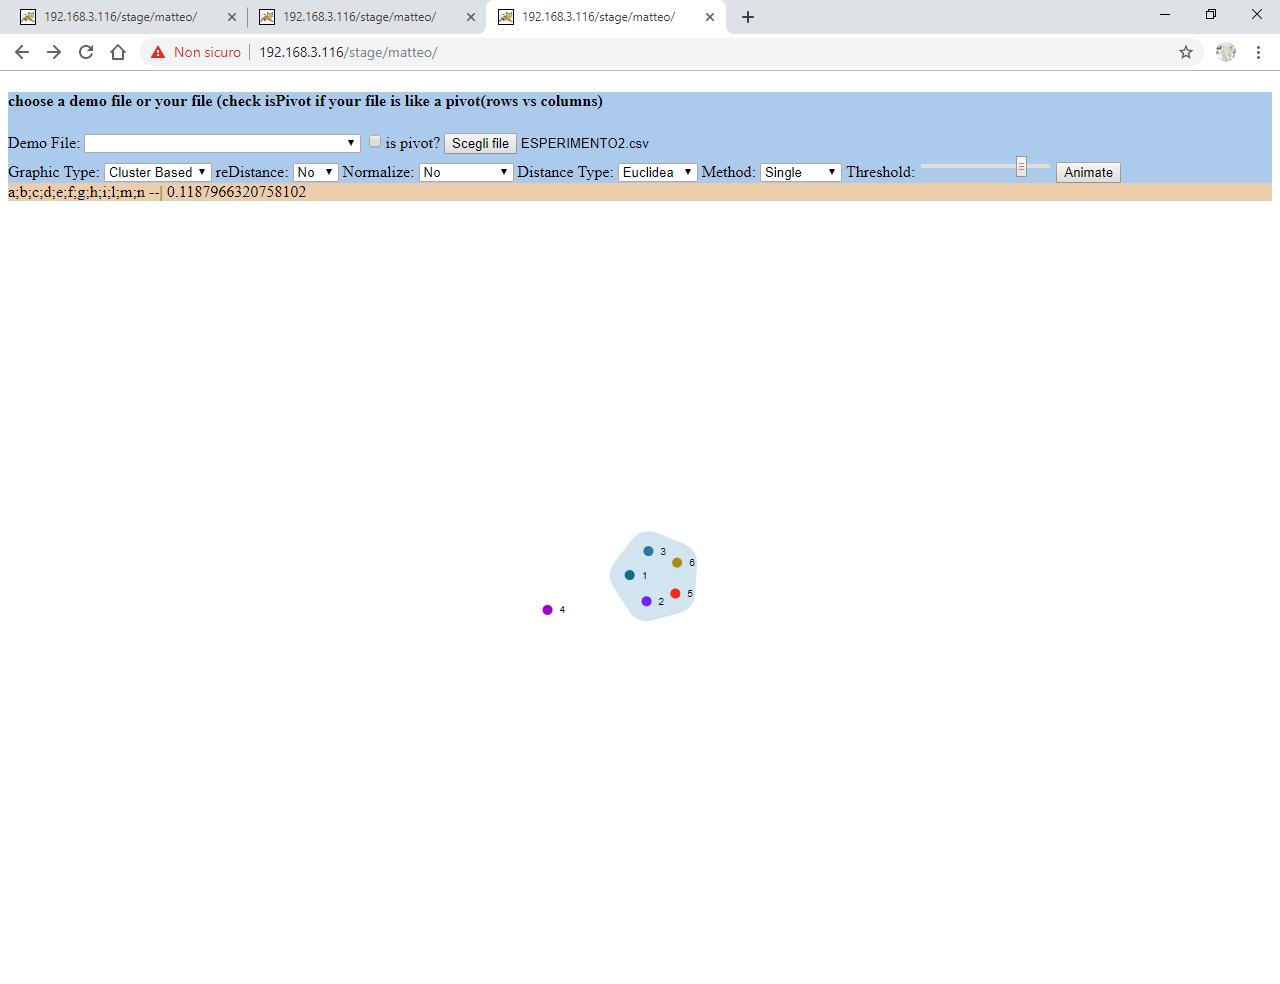
\includegraphics[width=1\linewidth]{./image/reticoloNonCorretto3.png}
	\caption{Reticolo della Conoscenza con rappresentazione di tipo Cluster Based - 2.}
	\label{Reticolo della Conoscenza con rappresentazione di tipo Cluster Based - 2.}
\end{figure}
\noindent
\begin{figure}[H]
\centering
	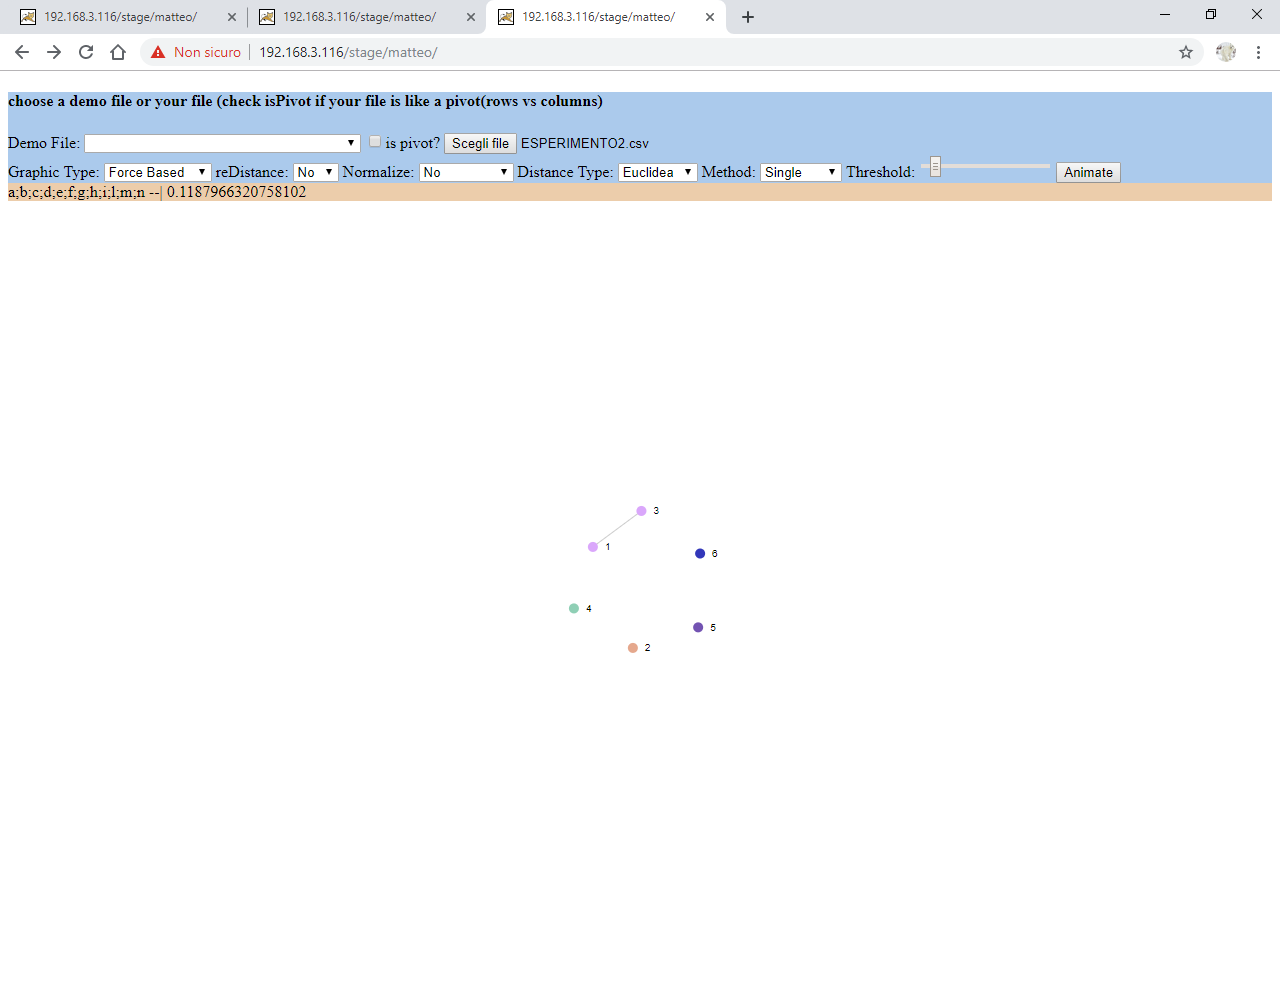
\includegraphics[width=1\linewidth]{./image/reticoloNonCorretto4.png}
	\caption{Reticolo della Conoscenza con rappresentazione di tipo Cluster Based - 3.}
	\label{Reticolo della Conoscenza con rappresentazione di tipo Cluster Based - 3.}
\end{figure}
\noindent
\begin{figure}[H]
\centering
	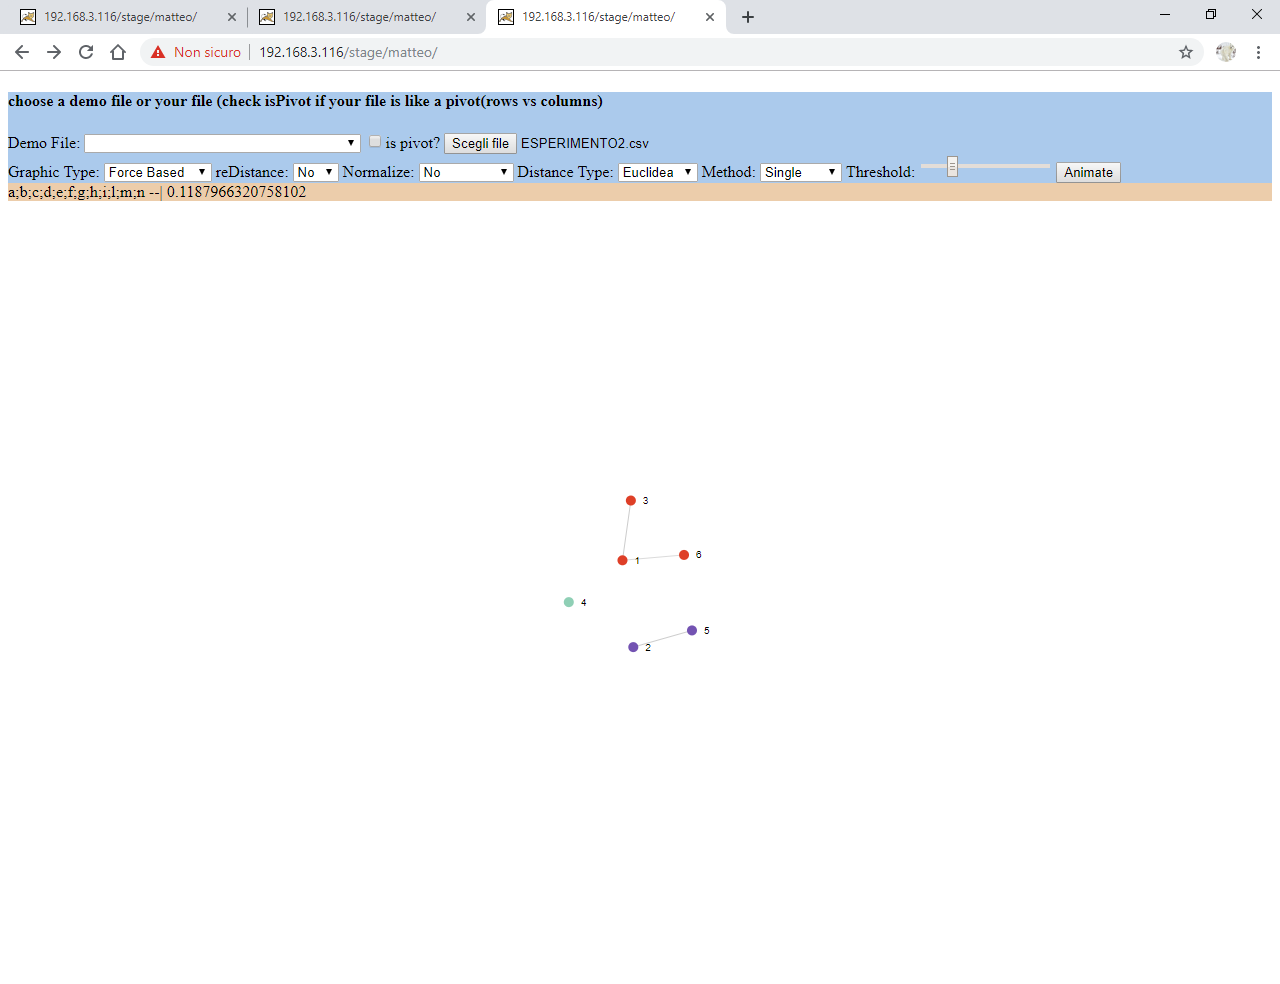
\includegraphics[width=1\linewidth]{./image/reticoloNonCorretto5.png}
	\caption{Reticolo della Conoscenza con rappresentazione di tipo Forced Based - 1.}
	\label{Reticolo della Conoscenza con rappresentazione di tipo Forced Based - 1.}
\end{figure}
\noindent
\begin{figure}[H]
\centering
	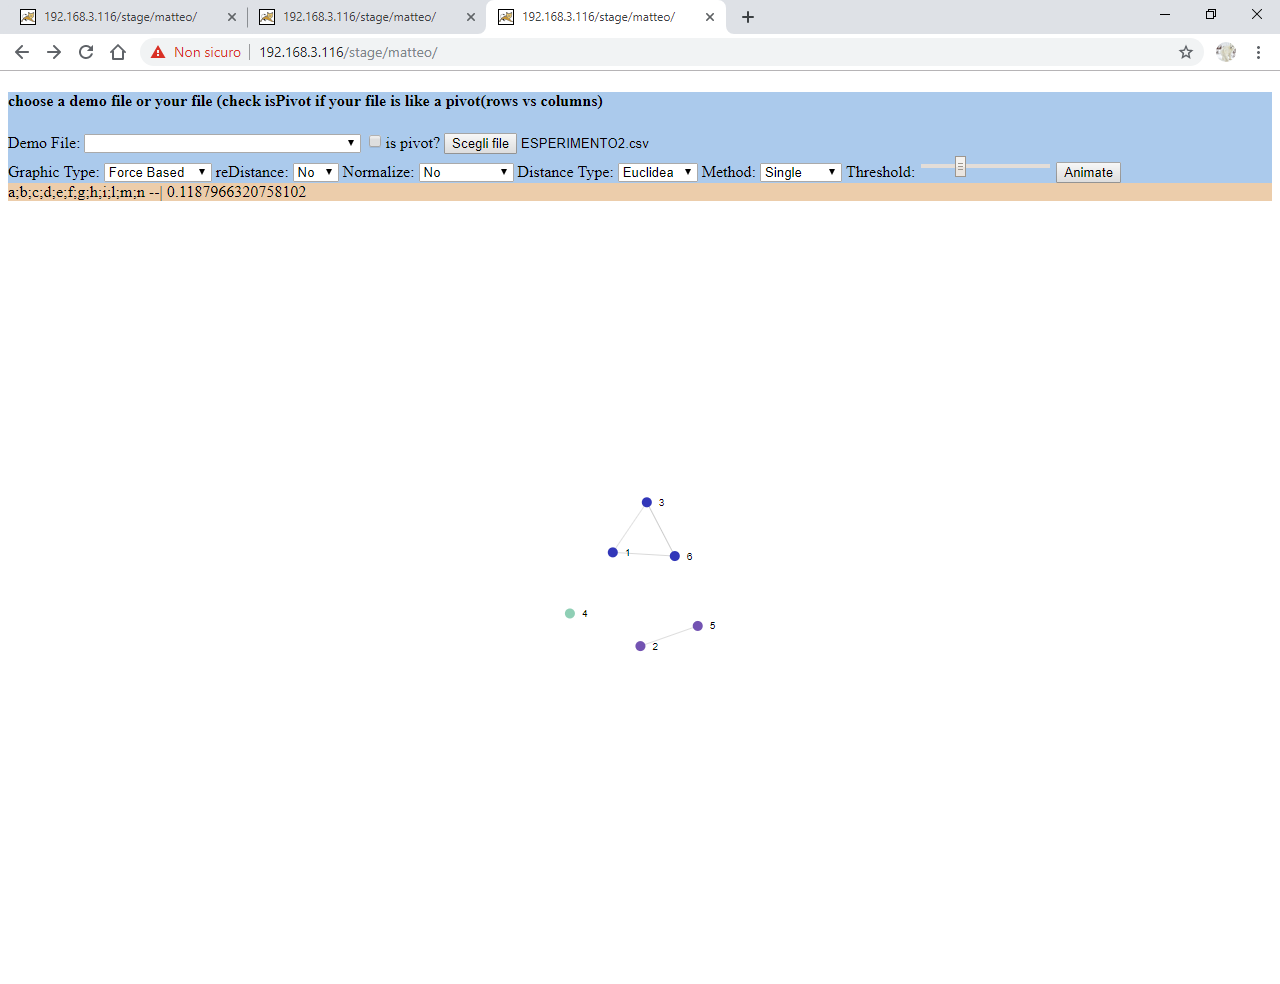
\includegraphics[width=1\linewidth]{./image/reticoloNonCorretto6.png}
	\caption{Reticolo della Conoscenza con rappresentazione di tipo Forced Based - 2.}
	\label{Reticolo della Conoscenza con rappresentazione di tipo Forced Based - 2.}
\end{figure}
\noindent
\begin{figure}[H]
\centering
	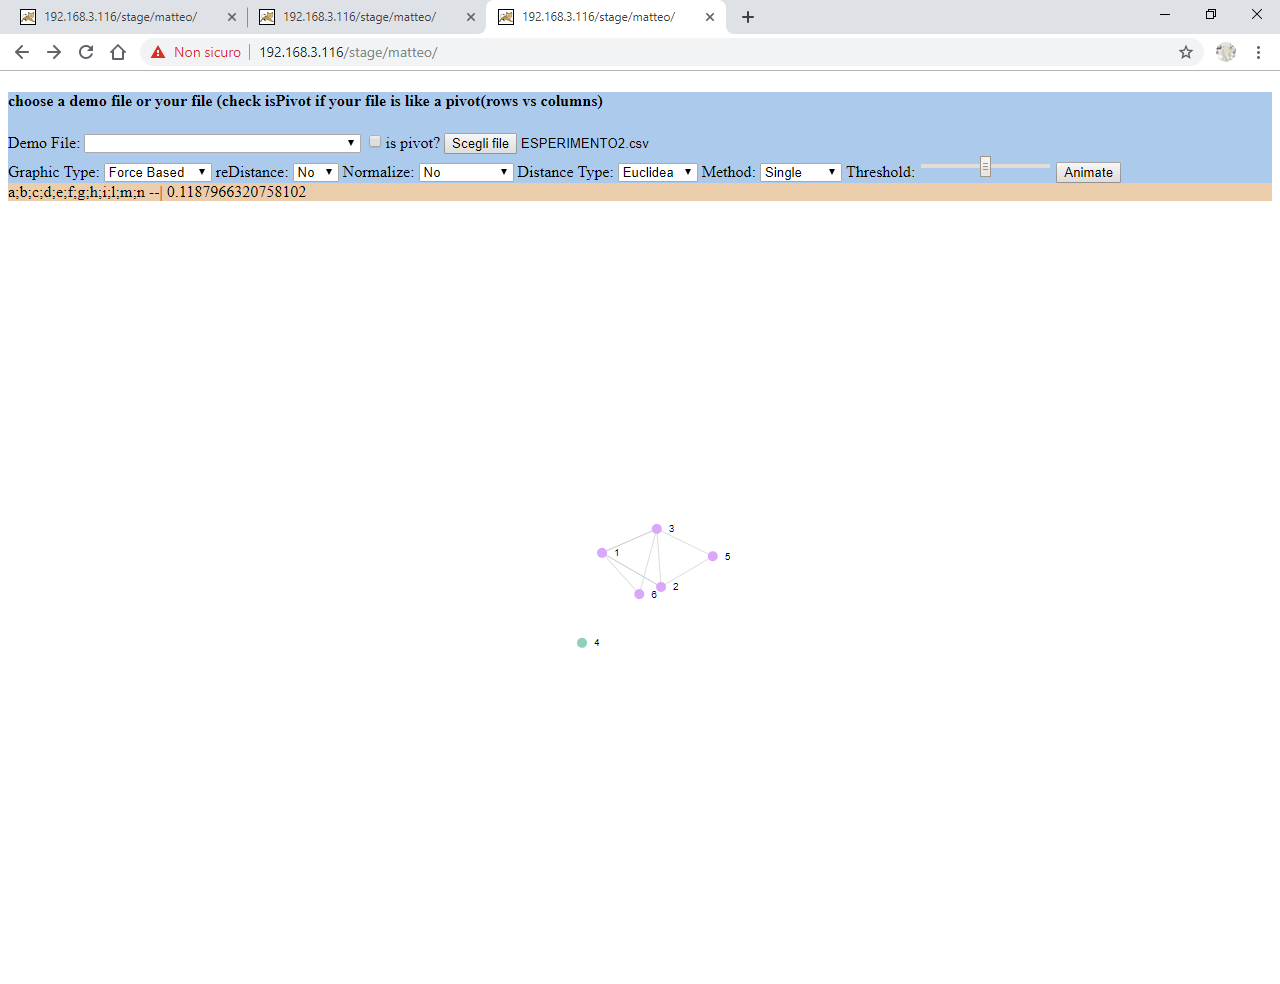
\includegraphics[width=1\linewidth]{./image/reticoloNonCorretto7.png}
	\caption{Reticolo della Conoscenza con rappresentazione di tipo Forced Based - 3.}
	\label{Reticolo della Conoscenza con rappresentazione di tipo Forced Based - 3.}
\end{figure}
\noindent
\begin{figure}[H]
\centering
	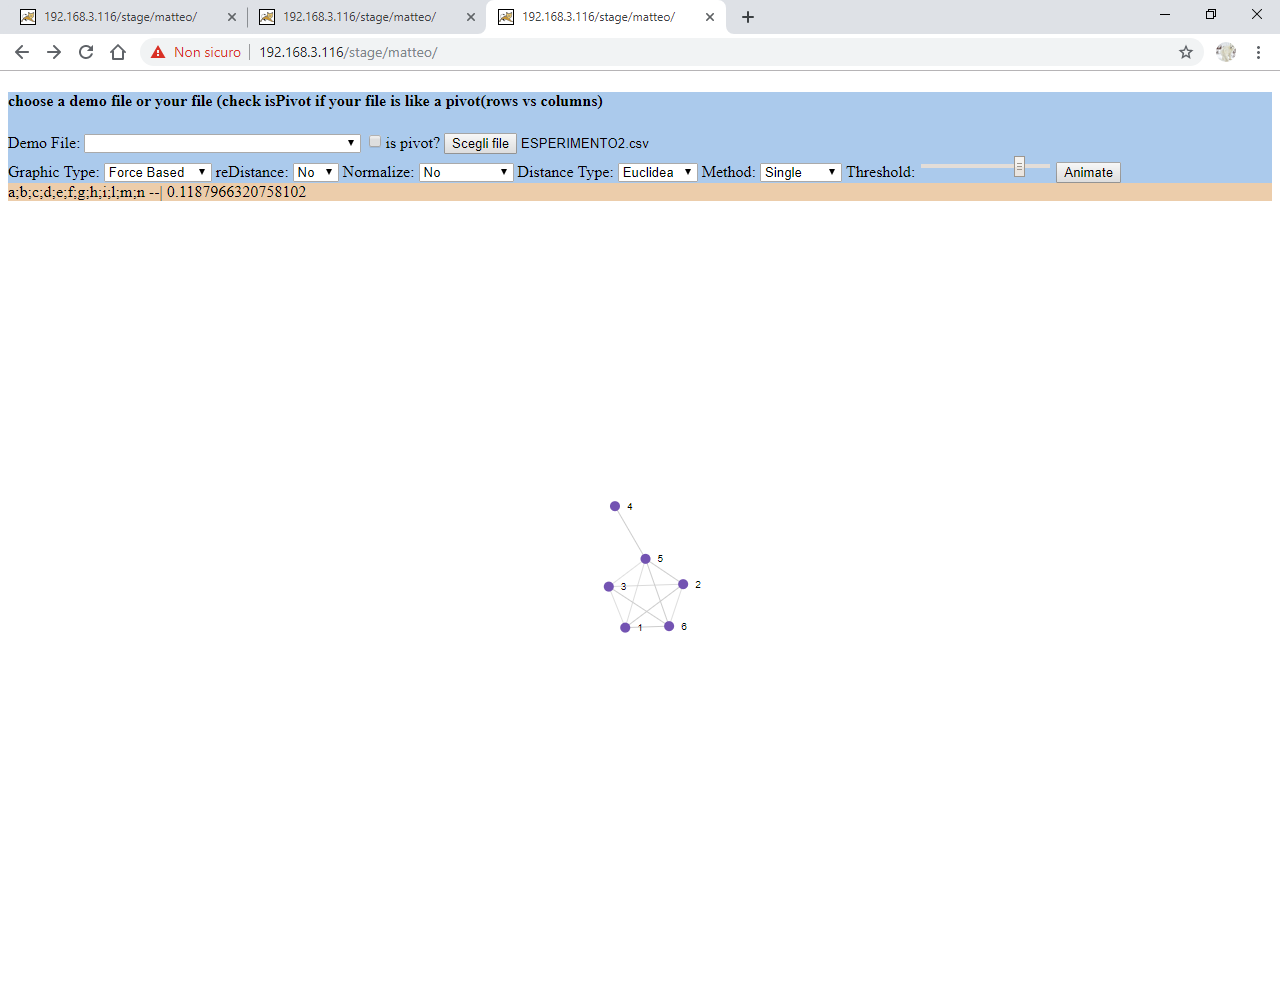
\includegraphics[width=1\linewidth]{./image/reticoloNonCorretto8.png}
	\caption{Reticolo della Conoscenza con rappresentazione di tipo Forced Based - 4.}
	\label{Reticolo della Conoscenza con rappresentazione di tipo Forced Based - 4.}
\end{figure}
\noindent
La spiegazione del Reticolo malformato sta nella natura di creazione dei dati di input.
\end{figure}
\noindent
\begin{figure}[H]
\centering
	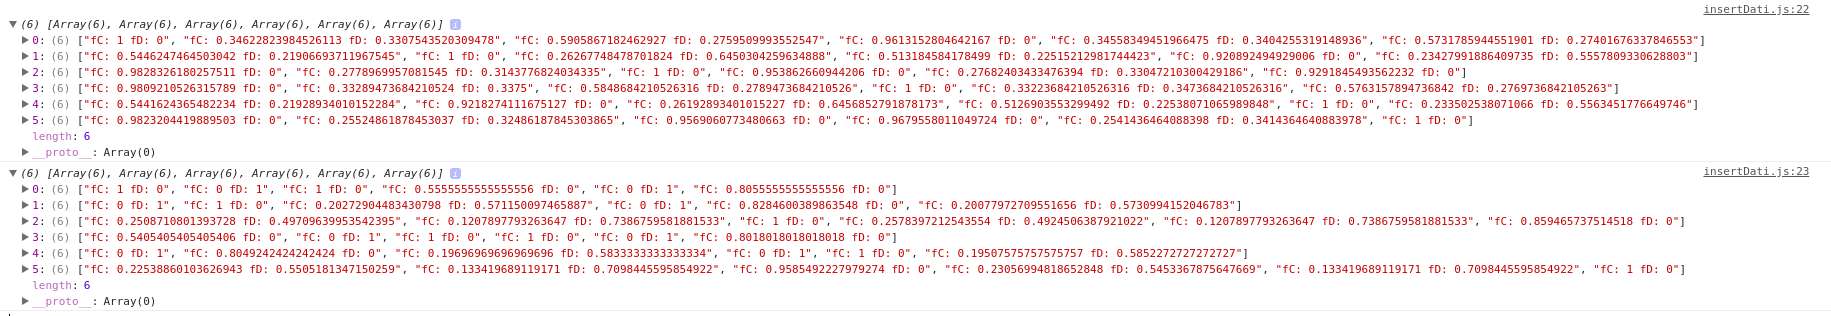
\includegraphics[width=1\linewidth]{./image/res_frequenceMatrix_OSS.png}
	\caption{Frequenza delle domande dei dati di test.}
	\label{Frequenza delle domande dei dati di test.}
\end{figure}
L'immagine sopra mostra per ogni domanda valutata a 1 (primo set di dati) e a -1 (secondo set di dati) la frequenza che intercorre in tutte le domande con segno coerente e opposto a quello della domanda in esame.
Il set di dati viene generato randomicamene con guida, ha infatti come traccia il Grafo della Conoscenza (mostrato in figura\ref{Grafo rappresentante le relazioni esistenti tra il set di domande di prova.}. \`E proprio la natura parzialmente randomica del set di dati che genera queste situazioni di incoerenza. La domanda 2 \`e positiva solo se lo \`e anche la domanda 5 
\noindent

\subsubsection{Osservazioni}
\subsubsection{Osservazioni Reticolo dati di prova}
Il Reticolo della Conoscenza \`e perfettamente coerente con le aspettative; ricalca fedelmente quanto evidenziato nella figura \ref{Grafo rappresentante le relazioni esistenti tra il set di domande di prova.} nella sezione § \ref{Test effettuati} Inoltre gli accoppiamenti tra i punti ricalcano quanto dichiarato dalla matrice correlazione ottenuta dal calcolo del modello effettuato con la PCA e visibile dall'immagine \ref{CSV generato a partire dalla matrice correlazione del trainset della rete di prova.}. Tuttavia i risultati della PCA non devo essere presi come assioma in quanto la Rete neurale, pu\`o cogliere oscillazioni che il modello matematico non \`e in grado.

\section{Creazione del Reticolo della Conoscenza sui dati delle domande nel database}
\label{Creazione del Reticolo della Conoscenza sui dati delle domande nel database}

\noindent
\begin{figure}[H]
\centering
	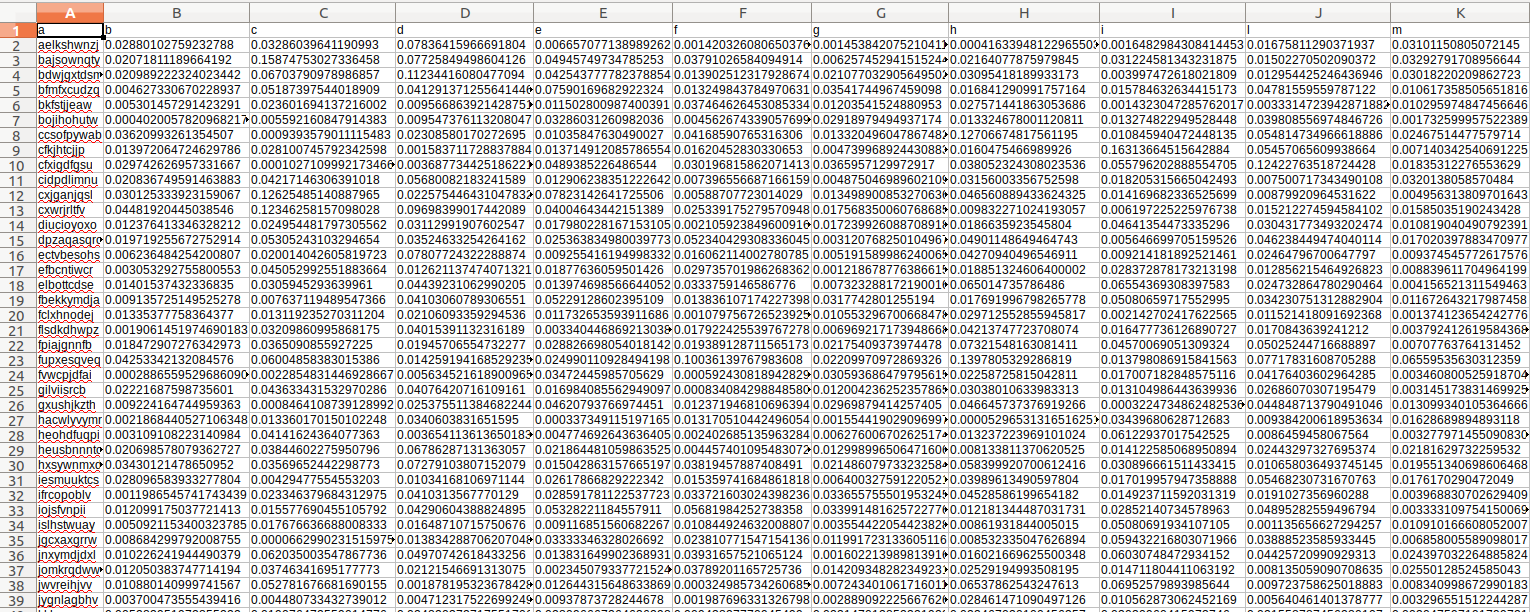
\includegraphics[width=1\linewidth]{./image/fileCSV_rete-db-10neuroni.png}
	\caption{Porzione di esempio file CSV generato per la creazione del Reticolo della Conoscenza sui dati del database.}
	\label{Porzione di esempio file CSV generato per la creazione del Reticolo della Conoscenza sui dati del database.}
\end{figure}
\noindent
La creazione del Reticolo della Conoscenza sui dati delle domande nel database ha richiesto la creazione di file CSV su un architettura a 2 layer della rete con 6, 8, 10, 12 neuroni ciascuno. Questo a causa della non conoscenza a priori del numero di cluster che comporranno il Reticolo, come invece accade per i dati di prova.\\
Tale differenziazione ha permesso durante la configurazione del sistema e la creazione del Reticolo che mi accorgersi dell'estrema variabilit\`a dei cluster e correlazioni a seconda dell'oscillazione del numero di neuroni per layers, come viene evidenziato dalle immagini seguenti.\\

TODO: INSERIMENTO DEI SCREEN DEL RETICOLO SUI CASI A 6, 8, 10, 12 NEURONI A CLUSTER E A FORCE BASED.

\subsection{Osservazioni}
\subsubsection{Osservazioni Reticolo dati del database}
La variazione dei Reticoli ottenuti dalle diverse architetture della Rete neurale indica come sia necessario approfondire la tematica e individuare una strategia unica che permetta di individuare in modo univoco l'architettura necessaria per ottenere un Reticolo della Conoscenza valido.



